% Created 2022-08-09 Tue 21:37
% Intended LaTeX compiler: pdflatex
\documentclass[11pt]{article}
\usepackage[utf8]{inputenc}
\usepackage[T1]{fontenc}
\usepackage{graphicx}
\usepackage{grffile}
\usepackage{longtable}
\usepackage{rotating}
\usepackage[normalem]{ulem}
\usepackage{amsmath}
\usepackage{textcomp}
\usepackage{amssymb}
\author{Alejandro Hervella, Peter Brown, Ian Chan, Gokce Saracoglu, Will Tower}
\date{\today}
\title{Capstone 1 Weekly Report}
\begin{document}

\maketitle
\tableofcontents



\section{Summary of Accomplishments}
\label{sec:org9ec5fd5}

\subsection{System Block Diagram}
\label{sec:orga1fc6db}
The group met to discuss research into various subsystems according to the previously established labor division, and produced a block diagram roughly defining subsystem interconnections.

\begin{center}
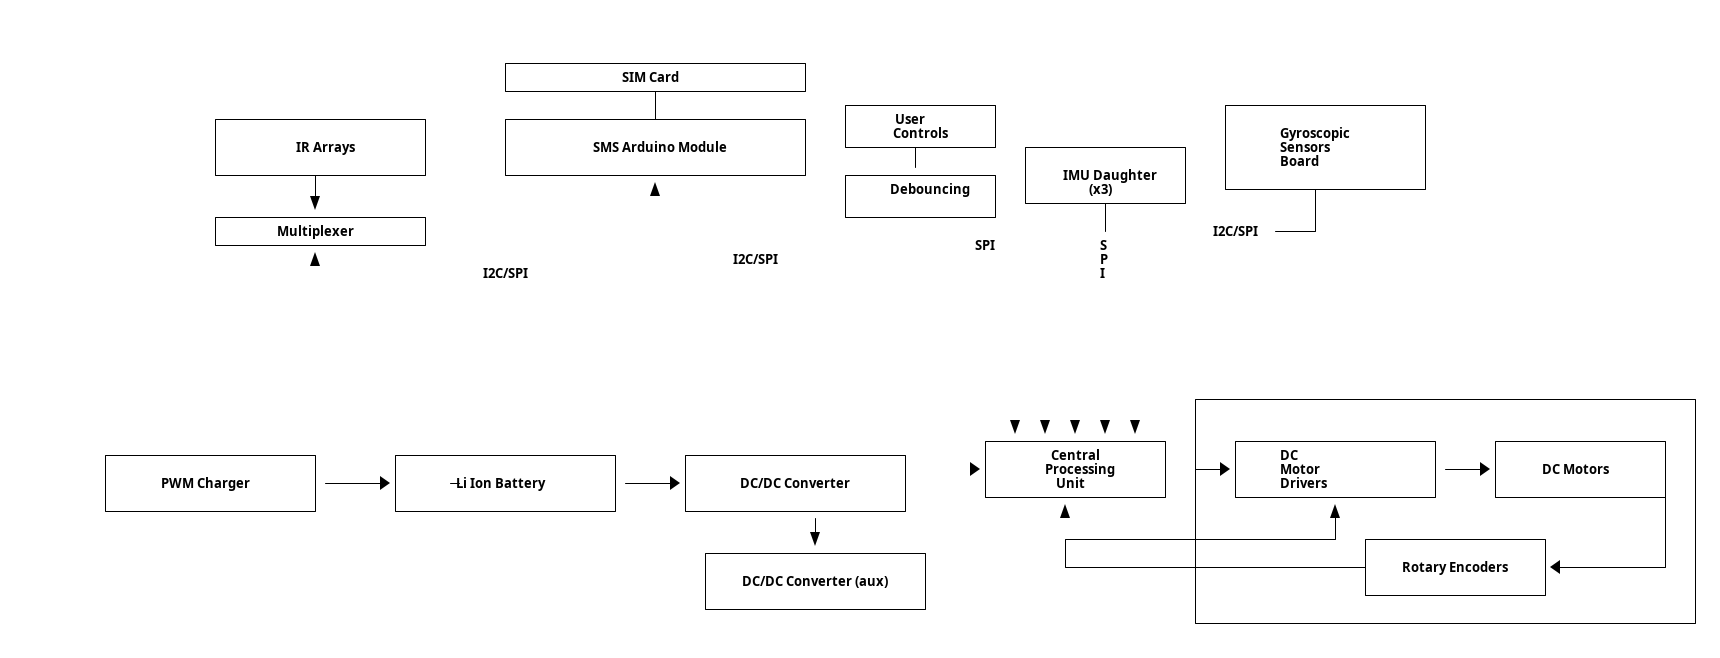
\includegraphics[width=1.2\linewidth]{block_diagram.png}
\end{center}


\subsection{Consultations}
\label{sec:org9ad63e6}
The group also contacted professor Andrew Gouldstone, setting a meeting Wednesday to discuss mechanical aspects of the project, and set a meeting with professor Padir the following Wednesday

\subsection{CAD work}
\label{sec:org6692719}
A STEP drawing of a use-case conversion wheelchair was produced in SolidWorks, to aid in analysis of weight distribution and the development of a retrofitting process.

\section{Next Week}
\label{sec:org9e78a51}

The group plans to meet with Taskin Padir, and spend a considerable amount of time developing and practicing our proposal presentation.
\end{document}